	\documentclass[14pt]{extreport}
\usepackage{extsizes}
	\usepackage[frenchb]{babel}
	\usepackage[utf8]{inputenc}  
	\usepackage[T1]{fontenc}
	\usepackage{amssymb}
	\usepackage[mathscr]{euscript}
	\usepackage{stmaryrd}
	\usepackage{amsmath}
	\usepackage{tikz}
	\usepackage[all,cmtip]{xy}
	\usepackage{amsthm}
	\usepackage{varioref}
	\usepackage[ margin=1in]{geometry}
	\geometry{a4paper}
	\usepackage{lmodern}
	\usepackage{hyperref}
	\usepackage{array}
	\usepackage{float}
	\usepackage{easytable}
\usepackage{stackengine}
	 \usepackage{fancyhdr}\usepackage{longtable}
	 \usetikzlibrary{shapes.misc}


\newcommand\xrowht[2][0]{\addstackgap[.5\dimexpr#2\relax]{\vphantom{#1}}}

	\pagestyle{fancy}
	\theoremstyle{plain}
	\fancyfoot[C]{\empty} 
	\fancyhead[L]{Contrôle}
	\fancyhead[R]{28 janvier 2025}
	
	
	\title{Contrôle chapitre 4}
	\date{}
	\begin{document}

\subsubsection*{Exercice 1 (8 points)}

Pour chaque liste de longueurs, peut-on construire un triangle ? Justifiez votre réponse pour chaque triangle. \begin{enumerate}
\item $AB = 3\text{ cm}, AC=9\text{ cm},BC = 4\text{ cm}$
\item $AB = 2\text{ cm}, AC=7\text{ cm},BC = 2\text{ cm}$
\item $AB = 13\text{ cm}, AC=8\text{ cm},BC = 4\text{ cm}$
\item $AB = 7\text{ cm}, AC=7\text{ cm},BC = 3\text{ cm}$
\end{enumerate}
\subsubsection*{Exercice 2 (6 points)}
 \begin{enumerate}
 \item Tracez un triangle avec $AB = 9$ cm, $AC = 8$ cm, et $BC = 6$ cm. 
 \item Tracez les trois médiatrices de ce triangle, et notez O leur point de concours. 
 \item Tracez le cercle passant par $A$, $B$ et $C$. 
 \item Tracez les trois hauteurs de ce triangle. 
 \end{enumerate}

\subsubsection*{Exercice 3 (4 points)}

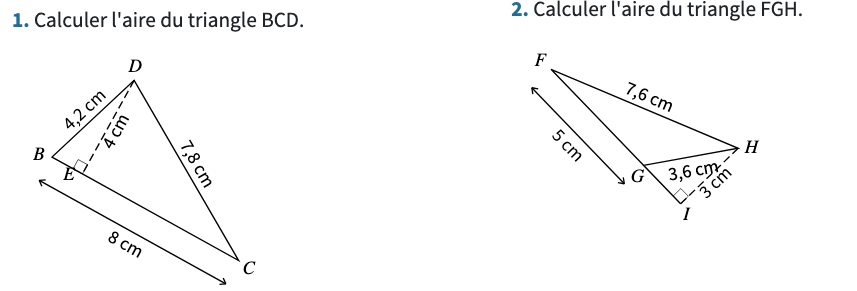
\includegraphics[scale=.45]{Exo3}
\subsubsection*{Exercice 4 (2 points)}
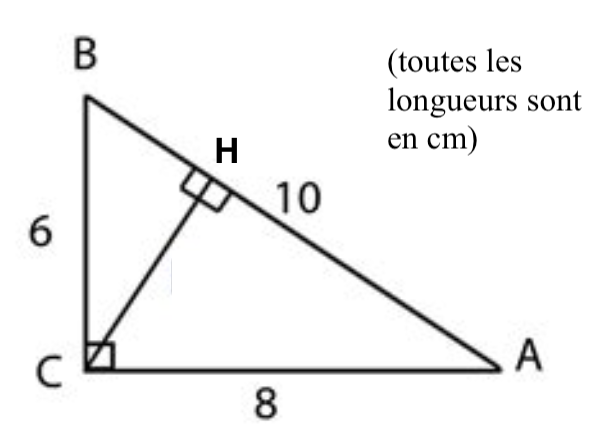
\includegraphics[scale=.45]{Exo4}\begin{enumerate}
\item Montrer que l'aire du triangle ABC est de $24$ cm${}^2$.
\item Exprimer d'une autre manière cette aire en fonction de la hauteur $HC$. 
\item En utilisant les questions précédentes, calculez la valeur de la hauteur $HC$. 
\end{enumerate}

\end{document}